\documentclass[tikz,border=0.1cm,usenames,dvipsnames]{standalone}
\usepackage{tikz,tikz-3dplot}
\usepackage{amsmath,amsthm}
\usepackage{amssymb}
\usepackage{amsfonts}
\usepackage{times}


\usetikzlibrary{positioning,arrows.meta,quotes}
\usetikzlibrary{shapes,snakes}
\usetikzlibrary{bayesnet}
\tikzset{>=latex}

\begin{document}
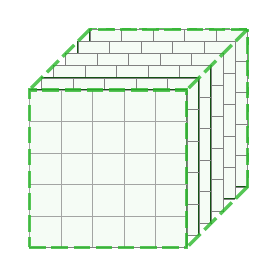
\begin{tikzpicture} 
    % Define the coordinates of the vertices
    \coordinate (A) at (0,0,0);
    \coordinate (B) at (2,0,0);
    \coordinate (C) at (2,2,0);
    \coordinate (D) at (0,2,0);
    \coordinate (E) at (0,0,2);
    \coordinate (F) at (2,0,2);
    \coordinate (G) at (2,2,2);
    \coordinate (H) at (0,2,2);
    \draw[thick,draw=LimeGreen!90!black, fill  opacity=0.3,fill=LimeGreen!5, draw opacity=0.8, dashed] (A) -- (B) -- (C) -- (D) -- cycle;
    \draw[thick,draw=LimeGreen!90!black, fill  opacity=0.3,fill=LimeGreen!5, draw opacity=0.8, dashed] (A) -- (E);
    
    % Draw 10 squares inside the cube along the z-axis
    \foreach \i in {0,...,5} {
        %\pgfmathsetmacro\offset{\i * 0.4} % Adjust the spacing between squares
        \begin{scope}[canvas is xy plane at z=\i*0.4]
            \draw[draw=LimeGreen!40!black, opacity=1.0, fill=LimeGreen!5] (0,0) rectangle (2,2);
            \draw[step=0.4, very thin, color=gray, opacity=1.0] (0,0) grid (2,2);
        \end{scope}
    }

    % Draw the edges of the cube
    \draw[thick,draw=LimeGreen!90!black, fill  opacity=0.3,fill=LimeGreen!5, draw opacity=0.8, dashed, line width=1.2pt, dash pattern=on 6pt off 2pt] (E) -- (F) -- (G) -- (H) -- cycle;
    \draw[thick,draw=LimeGreen!90!black, fill  opacity=0.3,fill=LimeGreen!5, draw opacity=0.8, dashed, line width=1.2pt, dash pattern=on 6pt off 2pt] (D) -- (H);
    \draw[thick,draw=LimeGreen!90!black, fill  opacity=0.3,fill=LimeGreen!5, draw opacity=0.8, dashed, line width=1.2pt, dash pattern=on 6pt off 2pt] (B) -- (F);
    \draw[thick,draw=LimeGreen!90!black, fill  opacity=0.3,fill=LimeGreen!5, draw opacity=0.8, dashed, line width=1.2pt, dash pattern=on 6pt off 2pt] (C) -- (G);
    \draw[thick,draw=LimeGreen!90!black, fill  opacity=0.3,fill=LimeGreen!5, draw opacity=0.8, dashed, line width=1.2pt, dash pattern=on 6pt off 2pt] (B) -- (C);
    \draw[thick,draw=LimeGreen!90!black, fill  opacity=0.3,fill=LimeGreen!5, draw opacity=0.8, dashed, line width=1.2pt, dash pattern=on 6pt off 2pt] (C) -- (D);

    %\draw[thin, draw=Gray, ->=, >=stealth'] (-0.25, 2, 2) -- (-0.25, 2, 0);

\end{tikzpicture}
\end{document}